% !TeX spellcheck = cs_CZ
\wikitextrule
\begin{example}\label{MAI:exam024} 
  Funkce $f:\,y=x^2$ je sudá, funkce $g:\,y=x^3$ je lichá.
  
  {\centering
   \begin{tabular}{cc}
     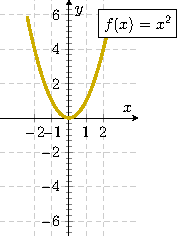
\includegraphics[width=0.5\linewidth]{mai_fig010.pdf}              &
     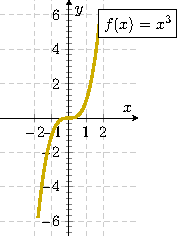
\includegraphics[width=0.5\linewidth]{mai_fig011.pdf}             \\
  \end{tabular}
  \captionsetup{type=figure}
  \captionof{figure}{Příklad sudé a liché funkce}\label{MAI:fig_002}
  \par}
\end{example}